%% manuscript produces a one-column, double-spaced document:
\documentclass[manuscript]{aastex}
%\documentclass[manuscript]{emulateapj}
%\documentclass[twocolumn]{article}
%\documentclass[twocolumn]{emulateapj}

%% preprint2 produces a double-column, single-spaced document:
%% Sometimes a paper's abstract is too long to fit on the
%% title page in preprint2 mode. When that is the case,
%% use the longabstract style option.

%% \documentclass[preprint2,longabstract]{aastex}

%% If you are submitting to a journal that translates manuscripts
%% into SGML, you need to follow certain guidelines when preparing
%% your macros. See the AASTeX v5.x Author Guide
%% for information.

\newcommand{\vdag}{(v)^\dagger}
\newcommand{\numt}{60}

%% You can insert a short comment on the title page using the command below.

%%\slugcomment{Not to appear in Nonlearned J., 45.}

%% If you wish, you may supply running head information, although
%% this information may be modified by the editorial offices.
%% The left head contains a list of authors,
%% usually a maximum of three (otherwise use et al.).  The right
%% head is a modified title of up to roughly 44 characters.
%% Running heads will not print in the manuscript style.

\shorttitle{Using Limb Brightening for Transit Timing}
\shortauthors{Schlawin et al.}

%% This is the end of the preamble.  Indicate the beginning of the
%% paper itself with \begin{document}.

\begin{document}

%% LaTeX will automatically break titles if they run longer than
%% one line. However, you may use \\ to force a line break if
%% you desire.

\title{Transit Timing in the UV:\\
     Taking Advantage of Limb brightening}

%% Use \author, \affil, and the \and command to format
%% author and affiliation information.
%% Note that \email has replaced the old \authoremail command
%% from AASTeX v4.0. You can use \email to mark an email address
%% anywhere in the paper, not just in the front matter.
%% As in the title, use \\ to force line breaks.

\author{E. Schlawin} 
\affil{Astronomy Department, Cornell University, Ithaca NY 14850}
\author{E. Agol}
\affil{Astronomy Department, University of Washington, Seattle, WA 98195}
\author{J. Lloyd}
\affil{Astronomy Department, Cornell University, Ithaca NY 14850}
\author{L. Walkowicz}
\affil{Astronomy Department,University of California at Berkeley,Berkeley, CA 94720}
\author{K. Covey\altaffilmark{1}}
\affil{Astronomy Department, Cornell University, Ithaca NY 14850}


%%\affil{Astronomy Department, Cornell University,
%%    Ithaca, NY 14853}

% PUT THIS BACK IN ONC YOU FIGURE OUT HOW TO MAKE IT NOT CONFLICT WITH TEXT
%\altaffiltext{1}{Hubble Fellow}

%% Mark off your abstract in the ``abstract'' environment. In the manuscript
%% style, abstract will output a Received/Accepted line after the
%% title and affiliation information. No date will appear since the author
%% does not have this information. The dates will be filled in by the
%% editorial office after submission.

\bibliographystyle{apj}

\begin{abstract}
\end{abstract}

%% Keywords should appear after the \end{abstract} command. The uncommented
%% example has been keyed in ApJ style. See the instructions to authors
%% for the journal to which you are submitting your paper to determine
%% what keyword punctuation is appropriate.

\keywords{extrasolar planets: transit timing --- stellar chromospheres}
%% Authors who wish to have the most important objects in their paper
%% linked in the electronic edition to a data center may do so by tagging
%% their objects with \objectname{} or \object{}.  Each macro takes the
%% object name as its required argument. The optional, square-bracket 
%% argument should be used in cases where the data center identification
%% differs from what is to be printed in the paper.  The text appearing 
%% in curly braces is what will appear in print in the published paper. 
%% If the object name is recognized by the data centers, it will be linked
%% in the electronic edition to the object data available at the data centers  
%%
%% Note that for sources with brackets in their names, e.g. [WEG2004] 14h-090,
%% the brackets must be escaped with backslashes when used in the first
%% square-bracket argument, for instance, \object[\[WEG2004\] 14h-090]{90}).
%%  Otherwise, LaTeX will issue an error. 

\section{Introduction}
Of the exoplanets so far discovered, more than \numt\ are known to transit their
host star. These planets, with their favorable orbital alignment,
allow for calculation of planetary radii, stellar radii and average
density. Very accurate timing of the transit may reveal even more
information about the planet. So called transit timing variation (TTV)
measurements (\citep{2005MNRAS.359..567A}) can reveal deviations from
Keplerian elliptical motion due to the tug of another planet or even a
satellite.

Previous transit timing has been done with optical and infrared
telescopes (\citep{2004ApJ...613L.153A}, \citep{2010A&A...510A.107M} &
add some more TTV papers?) The light curve of these transits is smooth
and therefore the exact time at which egress begins or ingress ends is
difficult to pin down precisely. Part of the reason for the curve's
smoothness is limb darkening of the star: due to the temperature
stucture of the star, which decreases in temperature with radius,
shallower radial components in the line of sight will appear
darker. At the limb, where the shallowest radial component is seen,
the photosphere is (??? K), whereas a straight line of sight goes to a
deeper radial component and is (??? K).

In this paper, we outline a method of observing that has the opposite
effect: stars are limb brightnened for some wavelengths. In
particular, any optically thin chromospheric emission line will be
brighter at the limb than in the center. Just as with a planetary
nebula, like the Ring Nebula, the limb of a shell of gas is brighter
at the edges. This is because the column density at the limb is much
larger at the limb than in the center. This is different from the effect of limb darkening, which has to do with the temperature structure of the star. Coincidentally, the chromosphere is slightly temperature inverted so the same effect that causes limb brightening for optical emission can cause limb brightening for optically thick chromospheric lines.

\citet{2009ApJ...701.1616A} point out that limb brightening could be
very useful for detection of transits of giant planets. One advantage
to photometry in limb brightened wavelenghts is that transits are
deeper overall than for both limb brightened and uniform disk
emission. This is because the planet cover a larger amount of the
emission. \citet{2009Apj...701.1616A} approximate the limb brightened
star as a uniform ring of emission and therefore the amount of light
the planet blocks is simply the fraction of the ring covered instead
of the fraction of areas. With their approximation, the maximum depth
of the transit=$(R_p/R_*)$ instead of the $(R_p/R_*)^2$
as expected for a uniform disk.

A better approximation for the transit depth is to compare the area of
the projected planet shadow on the star to the total area of the
curved stellar surface. If the scale-height of the chromosphere, $h$,
is much smaller than the size of the planet and star, $R_p, R_*$, then
we can treat the chromosphere as a geometrically thin hemisphere of
emission.  This limit has the problem that at the edge of the shell,
the surface brightness will be infinite; this is an example classic
fold-caustic.  However, when one integrates the surface brightness
over area, the total flux is finite, and thus this still proves to be
a useful approximation.

However, rather than integrating over surface brightness to compute
the transit depth, the depth of transit is simply the area of the 
hemisphere that is blocked by the planet, $A_t$, divided by the total
area of the hemisphere, $2\pi R_*^2$.

We can estimate the maximum depth of transit as follows from
Figure \ref{fig01}.  When the planet touches the edge of the star 
(second contact), as shown from an edge-on viewpoint in this figure,
then the length of the arc of the long axis of the shadow is
$R_*\theta$.  Now, the diameter of the planet is given by 
$2 R_p \approx R_*(1-\cos{\theta}) \approx \frac{1}{2} R_* \theta^2$,
where the latter approxmiation is valid for $\theta \ll 1$.
Solving for $\theta$, we find $\theta = 2\sqrt{R_p/R_*}$, so to
be valid we require $R_p/R_* \ll 1/4$.  Now, we can approximate
the shadow as an ellipse which will have a minor axis of $R_p$
and a major axis of $R_*\theta$, so we can approximate the
area of the shadow as $A_t = \pi \sqrt{R_pR_*} R_p$.  Thus,
the maximum depth of transit is given by 
\begin{equation} \label{depth_anal}
{A_t \over \pi R_*^2} = \frac{1}{2} \left({R_p \over R_*}\right)^{3/2}.
\end{equation}
Note that this is a different scaling than that given in Assef et 
al.\ (2009) who did not consider the fold-caustic nature of a chromospheric
transits.

This has the remarkable consequence that the depth of a chromospheric
transit does not decline as much with the radius of the planet as 
a transit of a uniform disk.  A chromospheric transit has a maximum
depth that is $\frac{1}{2} \left({R_* \over R_p}\right)^{1/2}$
times deeper than the maximum transit depth of a uniform disk;
thus smaller planets have an advantage to be observed at
chromospheric wavelengths, as emphasized by Assef et al.\ (2009).

\begin{figure}
%\centerline{\psfig{figure=Chromospheric_shadow.eps,width=4in}}
%\epsscale{3}
\includegraphics[trim = 1in 6in 2in 0.5in,clip,width=3 in]{Chromospheric_shadow.eps}
%\plotone{Chromospheric_shadow.eps}
\caption{Edge-on view of area of shadow cast by the planet
at the edge of the star.}
\label{fig01}
\end{figure}


 could be useful for
giant planets, but the scaling is different from their approximation
of (R$_p$/R$_*$).

-Transit Timing Variations \\
-\\
    Find the presence of other planets/moons and inclinations \citep{2005MNRAS.359..567A}. For example, using the Fast Inversion Method \citep{2010ApJ...709L..44N}\\
-\\
-\\    
-Limb Brightening \\
-\\
    How we can take advantage of optically thin chromospheric lines \\
-\\
-\\
    - We present a more detailed calculation in $\mathsection$\ref{labl:chromlcurve}
-\\
-\\
-\\

\section{Limb Brightening}
\label{labl:limbbright}
\subsection{Limb Brightened Lines}
-\\
Optically thin lines are the most limb-brightnened
-\\
-\\
For M Stars in the Near UV, we'd be looking at 
-\\
- FeII, SiII lines from 2300 \AA\  to 2775 \AA\ 
-\\
- Don't include the optically thick MgII h and k lines at
$\sim$2800 \AA\ \citep{2007PASP..119...67H}
-\\
-\\

\subsection{Chromospheric Light-Curve: Thin-Shell Approximation}
\label{labl:chromlcurve}

-\\
For optically thin chromospheric lines:
\begin{equation}
\delta_{\mathrm{LB}} = {A_t \over \pi R_*^2} \approx \frac{1}{2}\left( R_p/R_* \right)^{3/2}
\end{equation}
\begin{equation}
\delta_{\mathrm{UD}} = \left( \frac{R_p}{R_*} \right)^2
\end{equation}
where $\delta_{\mathrm{LB}}$ is the limb brightnened transit depth and
$\delta_{\mathrm{UD}}$ is the uniform disk transit depth \\
 -\\
 - Eric's figure: projection of planet shadow onto curved surface
 -\\ - \\

\subsection{Dependence on Planet Size}
-Chromospheric transit depths are deeper for the same size planet \\
-Chromospheric transit  depths for small planets are closer to the depths for large planets
 - Eric's figure: limb-brightnened vs. uniform-disk egresses for two different size planets \\
-Chromospheric transits allow you to look for transits of giant stars \\


\subsection{Isothermal Chromospheric Models}
- \\
- We use the coronal approximation (optical thinness of chromosphere)
- Eric's figure of a limb-brightned star \\
 - we assume an opaque photosphere which creates a discontinuity \\
- A more accurate prediction can made with an exponential emissivity \\
--- When the scale height is larger than the planet, it's a smoother, longer-lived transit \\
--- When the scale height is smaller than the planet, it gets sharper, but starts loosing flux when we can't see the emission from the far side \\


\subsection{Comparison to SOHO data}
-\\
- Compare our models to lightcurves from SOHO FeIX images
 (or lightcurves from STEREO observing the moon crossing the sun) \\
- explain discrepencies\\
- discuss differences between M-dwarf or giant chromoshperic transit
vs. a sun-like chromospheric transit \\

\section{The Effects of Stellar Activity}
-\\
-    Starspots - are they a problem? \\
-\\
-    Compare Transit lifetime to flare lifetimes
-  Select and list more quiescent stars that would be good candidates

\section{Signal to Noise Calculations}
- What does the NUV flux and (R$_p$/R$_*$) have to be to make this feasible?

\section{Targets for UV Observations}
- I think this is going to be M-dwarfs and giants \\
- stars where our method beats conventional photometry
-      Report GALEX fluxes \\
-   Possible telescopes - Swift, Hubble or GALEX \\

\subsection{Chromospheric Science}
- \\
- In addition to UV transit timing, we could also study chromospheres
- \\
- We can map out spots and even see how they might migrate as done by \citet{2010arXiv1002.4113H}

\section{Conclusion}
\bibliography{paper}
%%  \begin{figure}
%%  \epsscale{.80}
%%  %\plotone{f1.eps}
%%  \caption{Derived spectra for 3C138 \citep[see][]{heiles03}. Plots for all sources are available
%%  in the electronic edition of {\it The Astrophysical Journal}.\label{fig1}}
%%  \end{figure}
%%  
%%  \clearpage
%%  
%%  %% Here we use \plottwo to present two versions of the same figure,
%%  %% one in black and white for print the other in RGB color
%%  %% for online presentation. Note that the caption indicates
%%  %% that a color version of the figure will be available online.
%%  %%
%%  
%%  \begin{figure}
%%  %\plottwo{f2.eps}{f2_color.eps}
%%  \caption{A panel taken from Figure 2 of \citet{rudnick03}. 
%%  See the electronic edition of the Journal for a color version 
%%  of this figure.\label{fig2}}
%%  \end{figure}
%%  
%%  %% This figure uses \includegraphics to scale and rotate the still frame
%%  %% for an mpeg animation.
%%  
%%  \begin{figure}
%%  %\includegraphics[angle=90,scale=.50]{f3.eps}
%%  \caption{Animation still frame taken from \citet{kim03}.
%%  This figure is also available as an mpeg
%%  animation in the electronic edition of the
%%  {\it Astrophysical Journal}.}
%%  \end{figure}
%%  
  \end{document}
%%  
%%  %%
%%  %% End of file `sample.tex'.
